% !TEX encoding = UTF-8
% !TEX program = xelatex
\documentclass[pdf]{beamer}        
\usepackage{xeCJK,beamerthemesplit}
\usetheme{CambridgeUS}
\hypersetup{pdfpagemode=FullScreen} 
%\mode<presentation>{}

\title{在线购物网站}
\subtitle{设计文档}
\author{Jitang Zheng}
\date{\today}

\begin{document}

\frame{\titlepage}


\section[目录]{}

\frame{\tableofcontents}

\section{技术选型原则}
\frame{
  \frametitle{大的基本原则 }
  按照重要性排序
  \begin{itemize}
    \item<2-> 安全: 安全靠的是人,不是技术,但是完善的平台可以帮助麻瓜规避风险。
    \item<3-> 开放:尽可能选择开源技术,可以方便跟踪源码。
    \item<4-> 活跃度:主流的技术,用户参与度高。
    \item<5-> 横向扩展:性能瓶颈的时候,应该可以方便地堆机器,而非动代码。
    \item<6-> 便利:科技以人为本,编码应该是一件享受的事情。
  \end{itemize}
}

\section{功能列表}
\subsection{原则基础}
\subsection{For 用户}
\subsection{For 编辑组}
\subsection{For 网站管理员}
\subsection{For 系统管理员}


\section{整体架构}
\subsection{系统平台}
\frame
{
  \frametitle{操作系统:Ubuntu 没啥说的}
  Why?
  \begin{itemize}
    \item<2-> 用户量大,其中年轻人很多
    \item<3-> 软件包更新快,技术支持也好
    \item<4-> 主流的云主机都支持
  \end{itemize}
}

\frame
{
  \frametitle{自建机房还是云主机?}
  个人倾向于云主机托管
  \begin{itemize}
    \item<2-> 按用量付费,根据访问人数规律按时段调节服务器数量
    \item<3-> 树大好乘凉,大量的安全专家提供的默认设置
    \item<4-> 自己做网线?被ddos攻击了自己买巨贵无比的防火墙?
    \item<5-> 在线管理,从此不用辛苦跑机房了
    \item<6-> 各种监控服务,比如过载报警等
    \item<7-> 省钱啊
    \item<8-> 最诱人的:便于运维自动化,麻瓜也可以管理服务器
  \end{itemize}
}


\subsection{运维部署}
\begin{frame}
  \frametitle{部署}
  \begin{center}
	  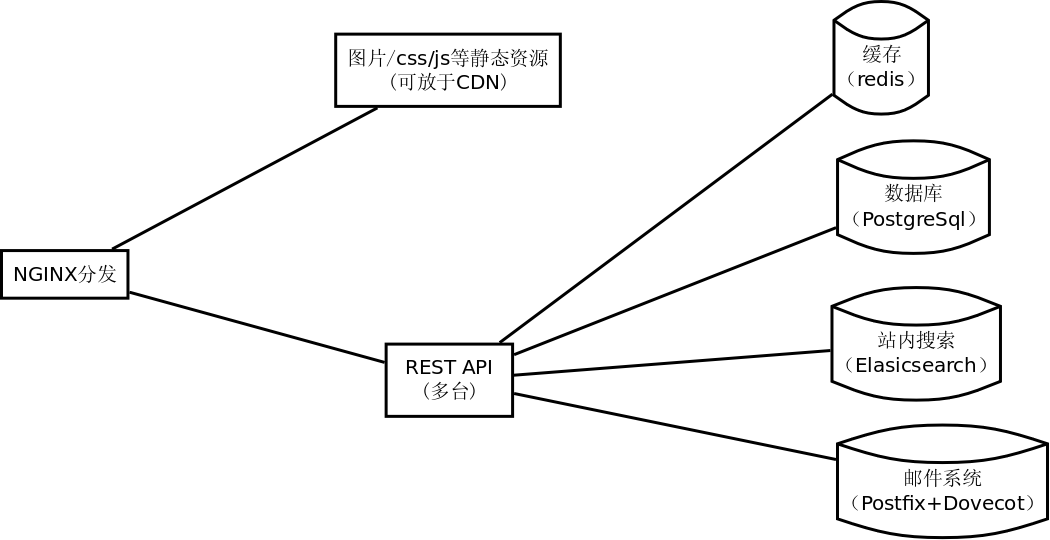
\includegraphics[width=1.0\textwidth]{1.png}
  \end{center}
\end{frame} 

\subsection{后端开发}
\begin{frame}
  \frametitle{JSON API}
  \begin{center}
	  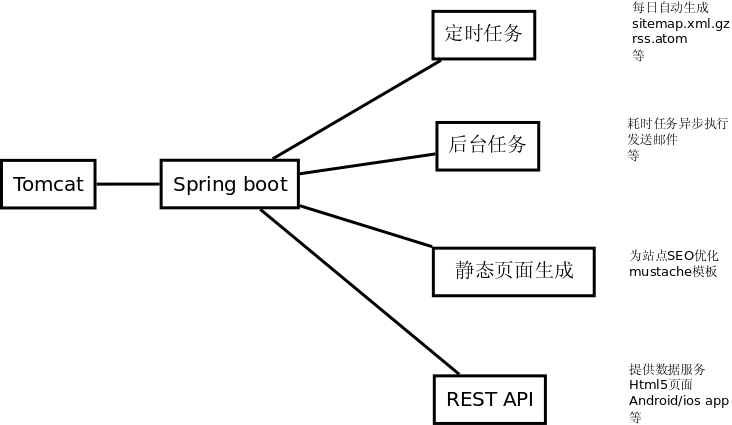
\includegraphics[width=1.0\textwidth]{2.png}
  \end{center}
\end{frame} 

\subsection{前端开发}
\begin{frame}
  \frametitle{SPA}
  \begin{center}
	  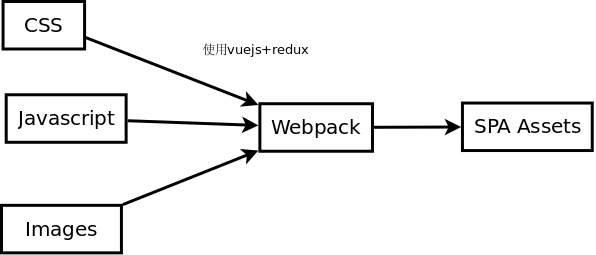
\includegraphics[width=1.0\textwidth]{3.png}
  \end{center}
\end{frame} 




\end{document}
